\section{Closing channels}

Often a component has to process a finite stream of data.  But how should the
end of the stream be signalled?  One way might be to send a special
``end-of-stream'' value.  But that assumes that we can find such a value,
namely a that won't be sent as a valid piece of data; and it will require
additional programming to send that value, and for the receiver to recognise
it and act appropriately.

Further, it can sometimes be useful for a receiver to indicate to the sender
that it is unable to accept any more data, which involves some form of
upstream signalling.

The way we deal with each of these scenarios is for the relevant thread to
close the channel. 
%
In SCL, if |in| is an |InPort| (e.g.~a channel), then |in.close()| closes it.
%
If |out| is an |OutPort| (e.g.~a channel), then |out.endOfStream()| closes it
for sending.  For a synchronous channel, this also closes it for receiving.
However, for a buffered channel, other threads can continue to receive until
the buffer becomes empty, at which point the channel becomes fully closed.

%%%%%

If a thread tries to send or receive on a channel that has been closed, it
throws a |Closed| exception, a subclass of the |Stopped| exception class.
(We will see another subclass of |Stopped| in Chapter~\ref{chap:alts}.)

Threads should normally catch such exceptions (see Scala
box~\ref{sb:try-catch}), and then do the right thing.  For a receiver, if the
closing represents the end of the data stream, then typically the thread
should terminate.  But if the thread is part of a larger network, such as a
pipeline, then typically the thread should first close channels to other
components, to signal to the next component in line that the stream is closed.

%% If such closing is possible, the thread should handle it appropriately,
%% normally closing its channels to pass the message on. 

\pagebreak[3]

Here's a new version of |alts| that does this.
%
\begin{mysamepage}
\begin{scala}
  def alts[A](in: ??[A], out: !![A]) = thread("alts"){ 
    try{ while(true){ out!(in?()); in?() } } 
    catch{ case _: Closed => in.close(); out.endOfStream() }
  }
\end{scala}
\end{mysamepage}
% 
If either sending or receiving fails, because the channel has been closed,
that operation throws a |Closed| exception, which is caught.  The overall
effect is that the thread exits the loop, and closes both channels.  
%
Note that closing a channel that is already closed has no effect.
Note also that there's no need to close a channel that is about to go out of
scope and be garbage collected. 

The above pattern is sufficiently common, that there's a construct to capture
it.
%
\begin{scala}
  repeat{ <command> }
\end{scala}
%
behaves much like
\begin{scala}
  while(true){ <command> }
\end{scala}
but catches |Stopped| exceptions, and so terminates cleanly if
\SCALA{<command>} throws such an exception.  Figure~\ref{fig:BoundedMults4}
illustrates this for the |nats|, |alts| and |console| functions.
%% For example:
%% %
%% \begin{scala}
%% def alts[A](in: ??[A], out: !![A]) = thread{ 
%%   repeat{ out!(in?()); in?() } 
%%   in.close(); out.endOfStream()
%% }
%% \end{scala}

%%%%%

It's sometimes useful to exit a loop for some reason other than a channel
being closed.  The construct
%
\begin{scala}
  repeat(guard){ <command> }
\end{scala}
%
behaves much like
\begin{scala}
  while(guard){ <command> }
\end{scala}
but terminates cleanly if \SCALA{<command>} throws a \SCALA{Stopped}
exception.

%%%%%%%%%%

Figure~\ref{fig:BoundedMults4} illustrates the technique of closing channels
via a version of the multiples-of-four example that prints up to some maximum
value~|max|, and then terminates cleanly.  This works by inserting a new
component into the pipeline, to close down the network once a value greater
than |max| is reached, as illustrated below.
%
\begin{center}
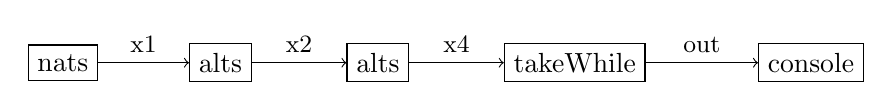
\begin{tikzpicture}
\draw (0,0) node[draw] (nats) {\scalashape nats};
\draw (nats)++(2,0) node[draw] (alts1) {\scalashape alts};
\draw[->] (nats) -- node[above]{\small\scalashape x1} (alts1);
\draw (alts1)++(2,0) node[draw] (alts2) {\scalashape alts};
\draw[->] (alts1) -- node[above]{\small\scalashape x2} (alts2);
\draw (alts2)++(2.5,0) node[draw] (takeWhile) {\scalashape takeWhile};
\draw[->] (alts2) -- node[above]{\small\scalashape x4} (takeWhile);
\draw (takeWhile)++(3,0) node[draw] (console) {\scalashape console};
\draw[->] (takeWhile) -- node[above]{\small\scalashape out} (console);
%
%% \draw (nats)++(1,-0.5) node {\small\scalashape 0};
%% \draw (nats)++(1,-1) node {\small\scalashape 1};
%% \draw (nats)++(1,-1.5) node {\small\scalashape 2};
%% \draw (nats)++(1,-2) node {\small\scalashape 3};
%% \draw (nats)++(1,-2.5) node {\small\scalashape 4};
%% \draw (nats)++(1,-3) node {\small\scalashape \vdots};
%% %
%% \draw (alts1)++(1,-0.5) node {\small\scalashape 0};
%% \draw (alts1)++(1,-1.5) node {\small\scalashape 2};
%% \draw (alts1)++(1,-2.5) node {\small\scalashape 4};
%% \draw (alts1)++(1,-3) node {\small\scalashape \vdots};
%% %
%% \draw (alts2)++(1,-0.5) node {\small\scalashape 0};
%% \draw (alts2)++(1,-2.5) node {\small\scalashape 4};
%% \draw (alts2)++(1,-3) node {\small\scalashape \vdots};
\end{tikzpicture}
\end{center}

%%%%%

\begin{figure}
\begin{scala}
object BoundedMults4{
  def nats(max: Int, out: !![Int]) = thread("nats"){ 
    var n = 0
    repeat{ out!n; n += 1 }
  }

  def alts[A](in: ??[A], out: !![A]) = thread("alts"){ 
    repeat{ out!(in?()); in?() }
    in.close(); out.endOfStream()
  }

  def console[A](in: ??[A]) = thread("console"){ repeat{ println(in?()) } }

  def takeWhile[A](p: A => Boolean, in: ??[A], out: !![A]) = thread("takeWhile"){
    var done = false
    repeat(!done){ val x = in?(); if(p(x)) out!x else done = true }
    in.close(); out.endOfStream()
  }

  def system(max: Int) = {
    val x1, x2, x4, out = new SyncChan[Int]
    nats(max, x1) || alts(x1, x2) || alts(x2, x4) || 
      takeWhile((x: Int) => (x <= max), x4, out) || console(out)
  }

  def main(args: Array[String]) = {
    val max = args(0).toInt; run(system(max))
  }
}
\end{scala}
\caption{Printing multiples of four, up to some maximum value.}
\label{fig:BoundedMults4}
\end{figure}

%%%%%

In fact, the new component is an instance of a more general pattern.  The
function |takeWhile(p, in, out)| copies data from~|in| to~|out| while all
values satisfy the predicate~|p| (the type \protect\SCALA{A => Boolean}
represents functions from~{\scalashape A} to~{\scalashape Boolean}; see Scala
box~\ref{sb:function-types}); it then closes the channels.

The other components are adapted to handle the closing of channels, using
|repeat|.  The |alts| components also close their channels, to indicate to
their neighbours that the system is terminating (in fact, the
``|out.endOfStream()|'' is unnecessary in this case because that part of the
network is closing in an upstream direction). 

The function |system| creates the channels and puts the components together in
parallel.  (In the first parameter of |takeWhile|, the notation \SCALA{(x:
  Int) => (x <= max)} represents the function that takes an |Int|
argument~|x|, and returns the result of the test |(x <= max)|; see Scala
box~\ref{sb:anon-function}.  In fact, the
parentheses around that test aren't necessary.)

\begin{instruction}
Make sure you understand how the termination signal is propagated through the
system. 
\end{instruction}
%\medskip

There are two other operations on channels related to closing. 
It is possible to test whether a channel~|c| is closed using the expression
%
\begin{scala}
  c.isClosed
\end{scala}
%
A closed channel~|c| can be reopened using the construct
\begin{scala}
  c.reopen()
\end{scala}
%
This has a precondition that the channel is indeed closed, and that no thread
is trying to send or receive on it.  This allows channels to be reused.

% \framebox{Cut above?}

%%%%%%%%%%%%%%%%%%%%%%%%%%%%%%%%%%%%%%%%%%%%%%%%%%%%%%%

\section{Example: producing the natural numbers}

We now consider another example of fine-grained concurrency, a circuit that
outputs the natural numbers.  The circuit is depicted below, and the code is
in Figure~\ref{fig:NatsCircuit}. 

\begin{center}
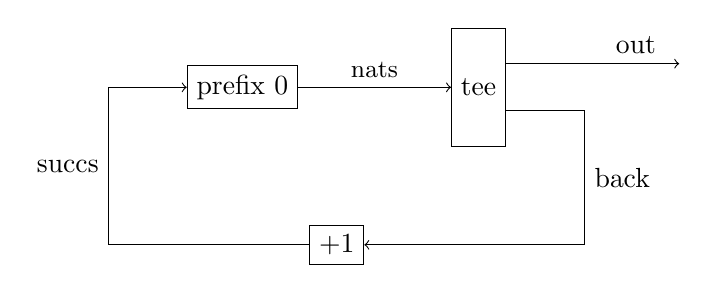
\begin{tikzpicture}
\draw(0,0) node[draw] (prefix) {\scalashape prefix 0};
% tee
\draw(prefix) ++(3,0) node[draw, minimum height = 15mm] (tee) {\scalashape tee};
\draw[->] (prefix) -- node[above]{\small\scalashape nats} (tee);
\draw[->] (tee.east)++(0,0.3) -- 
  node[above, near end]{\scalashape out} ++ (2.2,0);
% +1
\draw(prefix) ++ (1.2,-2) node[draw] (succ) {\scalashape +1};
\draw[->] (tee.east)++(0,-0.3) -- ++ (1.0,0) |-  
  node[right, near start]{\scalashape back} (succ);
\draw[->] (succ) -- ++(-2.9,0) |- 
  node[left, near start]{\scalashape succs} (prefix);
\end{tikzpicture}
\end{center}

%%%%%

\begin{figure}
\begin{scala}
object NatsCircuit{
  def console[A](in: ??[A]) = thread("console"){ repeat{ println(in?()) } }

  def prefix[A](x: A, in: ??[A], out: !![A]) = thread("prefix"){
    out!x; repeat{ out!in?() }
  }

  def tee[A](in: ??[A], out1: !![A], out2: !![A]) = thread("tee"){
    repeat{ val x = in?(); out1!x; out2!x }
  }

  def map[A,B](f: A => B, in: ??[A], out: !![B]) = thread("map"){
    repeat{ out!(f(in?())) }
  }

  def nats(out: !![Int]): ThreadGroup = {
    val nats, succs, back = new SyncChan[Int]
    prefix(0, succs, nats) || tee(nats, out, back) ||
      map(((x: Int) => x+1), back, succs)
  }

  def system: ThreadGroup = {
    val c = new SyncChan[Int]; nats(c) || console(c)
  }

  def main(args: Array[String]) = run(system)
}
\end{scala}
\caption{A concurrent circuit that outputs the natural numbers.}
\label{fig:NatsCircuit}
\end{figure}

The component labelled ``|prefix 0|'', produced using the function~|prefix|,
initially sends |0| on |nats|, and then copies values from |succs| to |nats|;
thus its output stream is its input stream prefixed by~|0|.  The component
labelled ``|tee|'', produced using the function~|tee|, copies values from
|nats| to both |out| and |back|.  The component labelled ``|+1|'' adds~|1| to
each value it receives on |back|, and outputs the result on |succs|; it is
produced by the function |map|, which generalises the particular functionality
we need, by applying the function~|f| to each value it receives.  Then |nats|
puts the components together, and |system| connects |nats| to a console
component.

Note that the circuit is cyclic.  Initially, |prefix 0| will produce~|0|; this
will be output and passed to |+1|.  The |+1| component will pass~|1| back to
|prefix 0|, via which it will be output and passed round the circuit.  And so
on.  In particular, it is important that |prefix 0| can send \emph{before} it
receives any value.  If every component started by trying to receive a value,
none would succeed, and the circuit would be deadlocked. 

\begin{instruction}
Make sure you understand how the circuit works, and how values propagate
round.
\end{instruction}

The above version of \SCALA{tee} outputs on its \SCALA{out1} channel before
its \SCALA{out2} channel.  That definition is fine in the context of the
circuit in question.  However, it could go wrong if used in the context of
some larger system that inputs on \SCALA{out2} before \SCALA{out1}.  For
example consider the following:
%
\begin{scala}
  val in, out1, out2 = new SyncChan[Int]
  def printer = thread("printer"){ println(out2?() + out1?()) } 
  run( tee(in, out1, out2) || printer)
\end{scala}
%
The printer thread will try to input on |out2| first (because |+| evaluates
its left-hand argument first).  But that means the system will get into a
deadlocked state, where the |tee| is blocked, trying to send on |out1|, and
the printer is blocked trying to receive on |out2|.  (Recall that in such
situations, typing \texttt{Ctrl}+$\backslash$ in the terminal produces a
thread dump, giving information about the running threads, which can be useful
for debugging.)

%% % %%%%%

%% Generic components should place as few assumptions as possible upon the
%% network in which they are placed. 
The following version of |tee| performs the outputs concurrently, which means
they can happen in either order.
%
\begin{mysamepage}
\begin{scala}
  def tee[A](in: ??[A], out1: !![A], out2: !![A]) = thread{
    repeat{ 
      val v = in?()
      run(thread{out1!v} || thread{out2!v}) 
    }
  }
\end{scala}
\end{mysamepage}
%
This version of |tee| will work fine in the context of the above system.  It
might be worth defining components in this style for generic components, or
when you don't know the order in which two communications will happen (and
this will be necessary in Exercise~\ref{ex:sorting}).  However, creating and
running two new threads is moderately expensive.  In specific settings, it
might be easier and more efficient to perform the outputs in a fixed order.
